

\chapter{Literature Review}

This chapter establishes the context of the research.

\section{Bird Recognition}

Birds are important indicators of the health of the environment. 
Birds  pollinate plants, disperse plant seeds and suppress pest populations. \citep{Farina2013}
The main method of bird monitoring is by point counts/field observation, tedious and time-consuming.
Many bird species are readily detectable by their sounds \citep{Kuaga2019}.
Bird sounds have been proven easy to collect \citep{Mcloughlin2019}.


Passive acoustic monitors (PAMs) left on site can continuously capture audio recordings and offer many advantages over field observers \citep{Digby2013,Sugai2019}.
 Recordings are retrieved manually, which can be days or weeks after the actual event.
The sounds are processed through spectrogram reading and/or listening by experienced observers.
It is not feasible to manually process weeks' or months’ worth of recordings. The trend today is towards automatic recognition \citep{Aide2013}.


\subsection{Audio Analysis of Bird Sounds}


\begin{table}
\centering
\caption{Sound event detection.}
\begin{tabular}{ccl}
\toprule
\textbf{Paper} & \textbf{Project} & \textbf{Contribution} \\
\midrule
\cite{Xie2018} & Frog Classification \\
\bottomrule
\end{tabular}
\end{table}

\begin{figure}
\centering
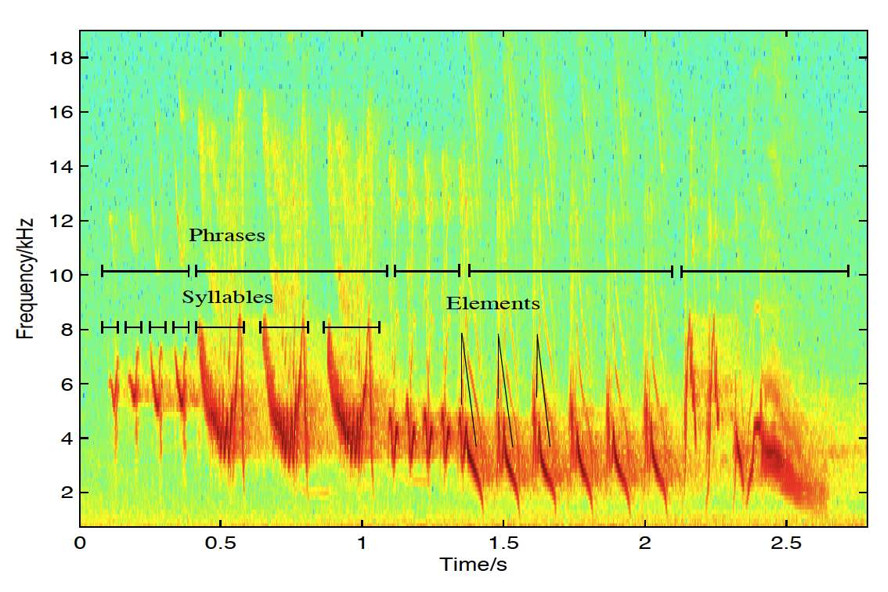
\includegraphics[scale=.33]{birdspectrogram}
\caption{Comparison of human and bird sound generation.}
\end{figure}

\begin{figure}[H]
\centering
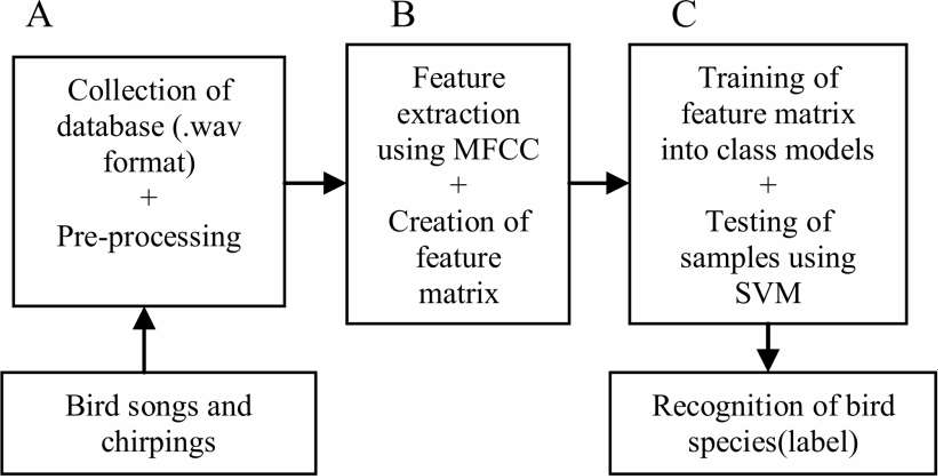
\includegraphics[scale=.33]{process}
\caption{process.}
\end{figure}

 The work presented in this article explores the automated method to identify bird species based on songs and calls of different bird species. This will help in archiving and identifying new species or subspecies. Moreover, it will help behavioral and ecological studies of birds and aid to the surveillance of bird population. In this work we implement a system that will be able to automatically identify bird species from acoustic recordings. Proposed system's ROC performance analysis shows that using Random Decision Tree we can yield 0.96 area under the curve.


Automatic bird classification based on their sound patterns is useful in the field of ornithology for studying bird species and their behavior based on their sound. The methodology may be used to conduct survey of birds. The methods may be used to automatically classify birds using different audio processing and machine learning techniques on the basis of their chirping patterns. This can then to map characteristics of birds such as size, habitat, species and types of call, on to their sounds.\cite{Raghuram2016}

\begin{table}
\renewcommand{\arraystretch}{.75}
\caption{Methods}
\centering
\small
\begin{tabular}{|l|c|c|}
\hline
\textbf{Technique}	&  \textbf{Accuracy} & \textbf{References} \\
\hline
Bayes net			& 69.90 			& \cite{Raghuram2016} \\
SVM 					& 70.75 -- 100 	& \cite{Raghuram2016}\cite{Zhao2017}\cite{Knapp2016} \\
NN 					& 78.60 			& \cite{Raghuram2016} \\
J-48 decision tree 	& 79.60 			& \cite{Raghuram2016} \\
Random forest 		& 83.88 			& \cite{Raghuram2016} \\
Wavelets + NN 		& 78 -- 96 		& \cite{Selin2007} \\
DNN 					& 88.5 -- 95.95	& \cite{Xie2019}\cite{Cakir2017} \\
\hline
\end{tabular}
\end{table}


\section{IoT and Edge Computing for Sound Event Detection}
	Recent advances in Internet of Things (IoT) enable novel kinds of applications and services including sound event recognition at the edge.
	Using IoT, passive audio sensors can transmit audio continuously to the cloud.
	However, cloud-based inference requires twice the energy compared to local processing \citep{Lane2016}
	Performing sound recognition at the point of occurrence enables faster response to the events and eliminate the need to transfer and process vast amounts of data.

	
\begin{figure}[H]
\centering
	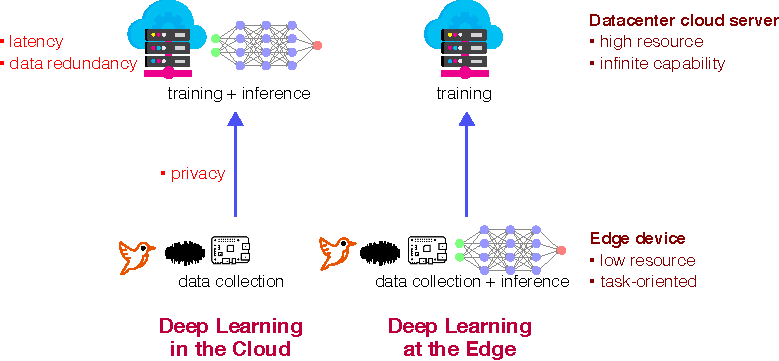
\includegraphics[width=.8\textwidth]{edgeinference}
	\caption{Cloud inference vs edge inference.}
\end{figure}


Two-stage classifiers achieve high accuracy at low power consumption for ASR applications \citep{Sigtia2018, Price2018, Yin2018}.
		 Not yet applied for bird recognition
		

\begin{figure}
\centering
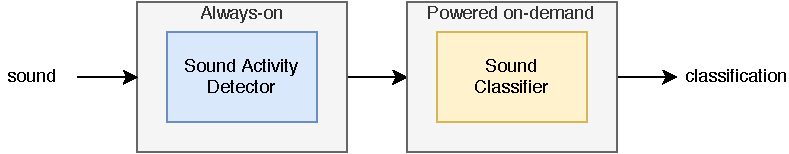
\includegraphics[width=.8\textwidth]{two-stage-classifier-gray}
\caption{Cascade audio classifier.}
\label{two-stage-classifier-gray}
\end{figure}

\FloatBarrier

\section{Deep Neural Networks}


\begin{figure}%[h]
\centering
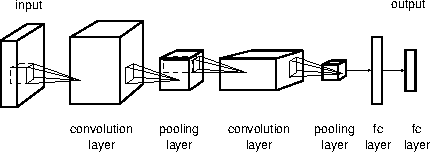
\includegraphics[scale=1.33]{typicalcnn}
\caption{An example of typical CNN with two convolution
layers, two pooling layers and two fully-connected (fc) layers.
Cubes are 3-D tensors and rectangular shapes are 1-D tensors,
and the relative tensor size presents actual data volume.}
\label{typicalcnn}
\end{figure}

\begin{figure}
\centering
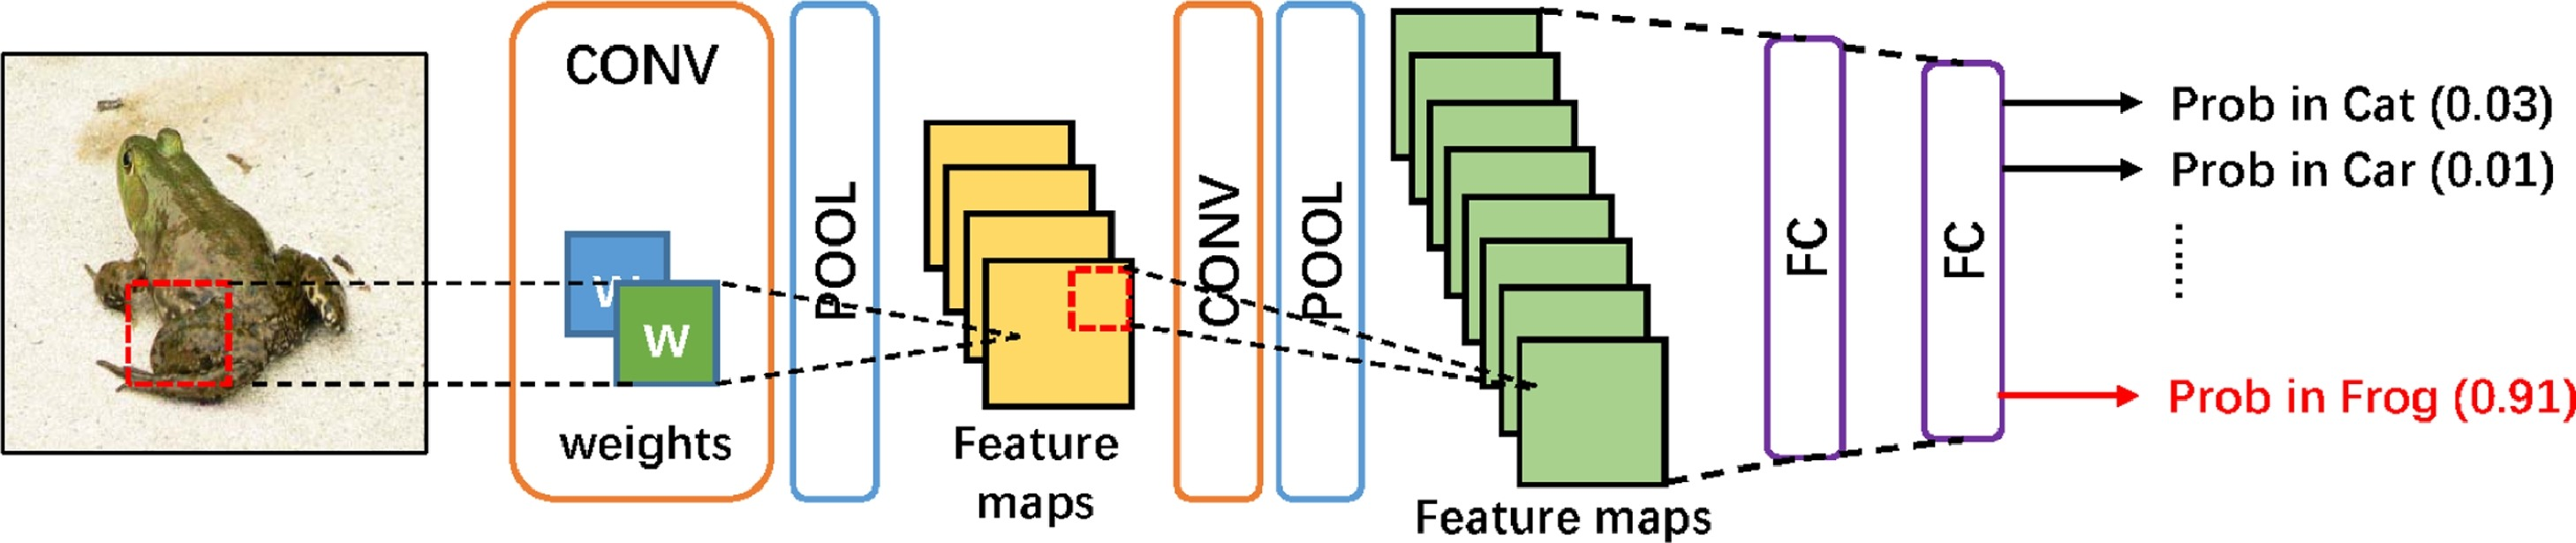
\includegraphics[width=.8\textwidth]{cnnbasic}
\caption{A typical CNN structure.}
\label{cnnbasic}
\end{figure}


%Chen2016
A typical CNN is illustrated in Fig. \ref{typicalcnn}. It is composed of three major layer types, (i) convolution, (ii) pooling, and (iii) fully-connected layers.

\subsubsection*{Convolution Layer}

A convolution layer extracts various features of local patches through massive convolution kernels and shares learned kernels among all spatial positions. By stacking multiple convolution layers, deep CNN delineates an input signal in different level of abstraction.

The convolution layer is computation-intensive layer and it requires high bandwidth to load data for massive convolutions. It convolves a 3D tensor (input, $\mathbf{X}\in \mathbb{R}^{C\times Y\times X}$) with 4D tensors (kernels, $\mathbf{X}\in \mathbb{R}^{N\times C\times H\times W}$) to extract different characteristics, then generates a 3D tensor (output, $\mathbf{Y}\in \mathbb{R}^{C\times Y'\times X'}$) where $C$, $Y$, $X$ are channel, height and width of input tensor, $C$, $H$, $W$ are channel, height and width of one convolution kernel and $N$ is number of convolution kernel, $N$, $Y'$ and $X'$ are channel, height and width of output tensor. Every convolution kernel produces one feature map of output tensor. By default (no padding and stride is one), $X' = X-W+1$ and $Y'=Y-H+1$. For a particular output feature point $(n,y,x)$, 

\[
y(n,y,x) = \sum^C_c\sum^H_j\sum^W_i X(c,y-j,x-i)*W(n,c,j,i)\
\]

\noindent
where $c$, $j$, and $i$ are indices of one of convolution kernels, and $n$ is the n-th convolution kernel. To generate all features, the following algorithm applies:

\begin{figure}
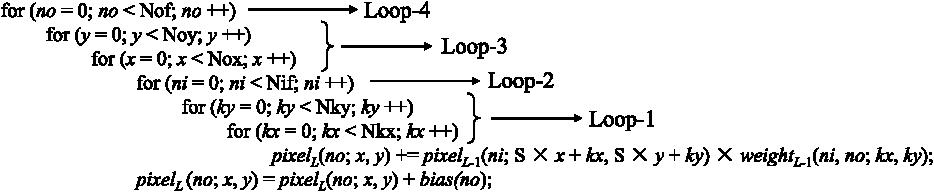
\includegraphics[width=\textwidth]{Ma2018}
\caption{Four levels of convolution loops, where $L$ denotes the index of convolution layer and $S$ denotes the sliding stride. }
\end{figure}


%\subsubsection*{CONV layer}
The CONV layer realizes a filter-like process, 
which uses a 
$K \times K$ weight kernel $W$
to convolve the input feature-map (fmap) 
$I$ in a sliding-window manner with a stride of $S$. This can be expressed as:

\[
A_n = B(n) + \sum_{m=1}^NW(m,n) \otimes I_m(i,j)
\]

\noindent 
where $\otimes$ is defined as convolution, which equal $K^2$ element-wise multiply-accumulates ($K$ is the kernel size):

\[
X \otimes Y = \sum_{i=1}^K\sum_{j=1}^KX(i,j)\cdot Y(i,j)
\]

\subsubsection*{Pooling Layer}

A pooling layer reduces the dimensionality expanded in convolution layers via fusing or selecting significant features in the spatial domain.
A pooling layer subsamples representative features in the spatial domain of every feature map, there
are two typical pooling operations, including average pooling
and maximum pooling. Average pooling computes the average
of given kernel as representative value. On the other hand,
maximum pooling derives the maximum value of given kernel
instead.

\subsubsection*{Fully-Connected Layer}

A fully-connected (FC) layer integrates mid-level features at different spatial locations into a high-level representation, and at the same time, the last fully-connected layer is the classifier to rank the possibility of each class.

A fully-connected layer fuses
locally extracted features from convolution layers into a highlevel representative, and fully-connected layer utilizes a linear
projection approach to map high-dimension feature vector to
dense but low-dimension feature vector. Computation of a
fully-connected layer can be expressed as matrix multiplication

\[
\mathbf{Y} = \mathbf{W^TX+b}
\]

\noindent 
where $\mathbf{W}\in \mathbb{R}^{M\times N}$ is weights of a fully-connected layer for fusing input features $\mathbf{X}\in \mathbb{R}^M$ to produce output $\mathbf{Y}\in \mathbb{R}^N$. $\mathbf{b}\in \mathbb{R}^N$ is a bias vector to increase non-linearity.

Table \ref{tabops} summarizes the number of operations required
by different layer types, a convolution layer requires heavy
computations among three layers due to massive convolution
kernels ($N$) and high tensor channels ($C$). On the other hand,
a fully-connected layer needs a huge storage size among all
layers when data volume of input ($M$) and output tensors ($N$)
are large.

\begin{table}
\centering
\caption{Number of operations of different layer type (\cite{Chen2016}).}
\label{tabops}
\begin{tabular}{cccc}
\toprule
\textbf{Layer type}	&	\textbf{Additions} &	\textbf{Multiplications} & \textbf{Weight Size} \\
\midrule
Convolution & $(C\times H\times W-1)\times N\times Y'\times X'$
			& $(C\times H\times W)\times N\times Y'\times X'$
			& $N\times C\times H\times W$ \\
Pooling		& $(H\times W-1) \times C \times Y'\times X'$
			& 0
			& 0 \\
Fully-connected	& $(M-1)\times N$
			& $M\times N$
			& $M\times N$ \\
\bottomrule				
\end{tabular}
\end{table}



Fig. \ref{cnnbasic} shows a typical CNN model (\cite{Liu2017}).
A CNN model usually consists of convolution (CONV) layer, dense (FC) layer and Pooling (POOL) layer, forming a trainable network. 


\subsubsection*{Activation layer}

Just like biological neurons, we say they are “firing” once the key value exceeds the threshold and are “silent” if not. Various activation functions are implemented in neural network designs to imitate the neurological behaviour such as ReLU, tanh, sigmoid, etc., which also introduce non-linearity to the networks.


\subsection{Database}

\cite{Vellinga2015}




\section{CNN}

While there has been extensive investigation on reducing
the complexity of well studied CNN models in the form
of parameter compression and quantization, there has
been limited effort on developing specialized CNN designs for bird species classification.
As such, in this work we focus on designing an
efficient and lightweight network to accelerate the execution of
the model with minimal compromise on the achieved accuracy

First, we adapted this basic model to detect only one class. Second, we explore the impact on performance by changing the structure of a CNN network such as the number of filters, the number of layers, the image size, the number of convolution and the pooling layers. Overall we design .... different structures


\subsection{CNN for Audio Recognition}


\cite{Pellegrini2017}


\subsection{Features}

\subsubsection*{MFCC}
MFCCs Mel-frequency cepstrum (MFC) is a represen- tation of the short-term power spectrum of a sound, based on a linear cosine transform of a log power spectrum on a nonlinear mel scale of frequency f as show in Eq. 4. Mel-frequency cepstral coefficients (MFCCs) are coefficients that collectively make up an MFC. The shape of the vocal tract manifests itself in the envelope of the short time power spectrum, and the job of MFCCs is to accurately represent this envelope.

The Mel-Frequency Cepstral Coefficients (MFCCs) are widely used in automatic speech recognition systems due to their low complexity estimation and their good performance. It has been demonstrated that the MFCC representation approximates the structure of human auditory system better than the traditional linear and predictive features. However, MFCC coefficients are easily affected by common frequency localized random perturbations, to which human perception is largely insensitive. For each frame of speech signal, a MFCC vector is computed as follows: the power of the spectrum of a windowed signal block is mapped onto the Mel scale using triangular filters. The logarithm of the filter bank output is then again transformed by applying a Discrete Cosine Transform (DCT). 

The relationship between scale Mel and frequency is given by the following expression


\[
\textit{Mel}(f) = 1125 \textit{ln} (1 + \frac{f}{700})
\]

\subsubsection{Spectrograms}

\begin{figure}[h]
\centering
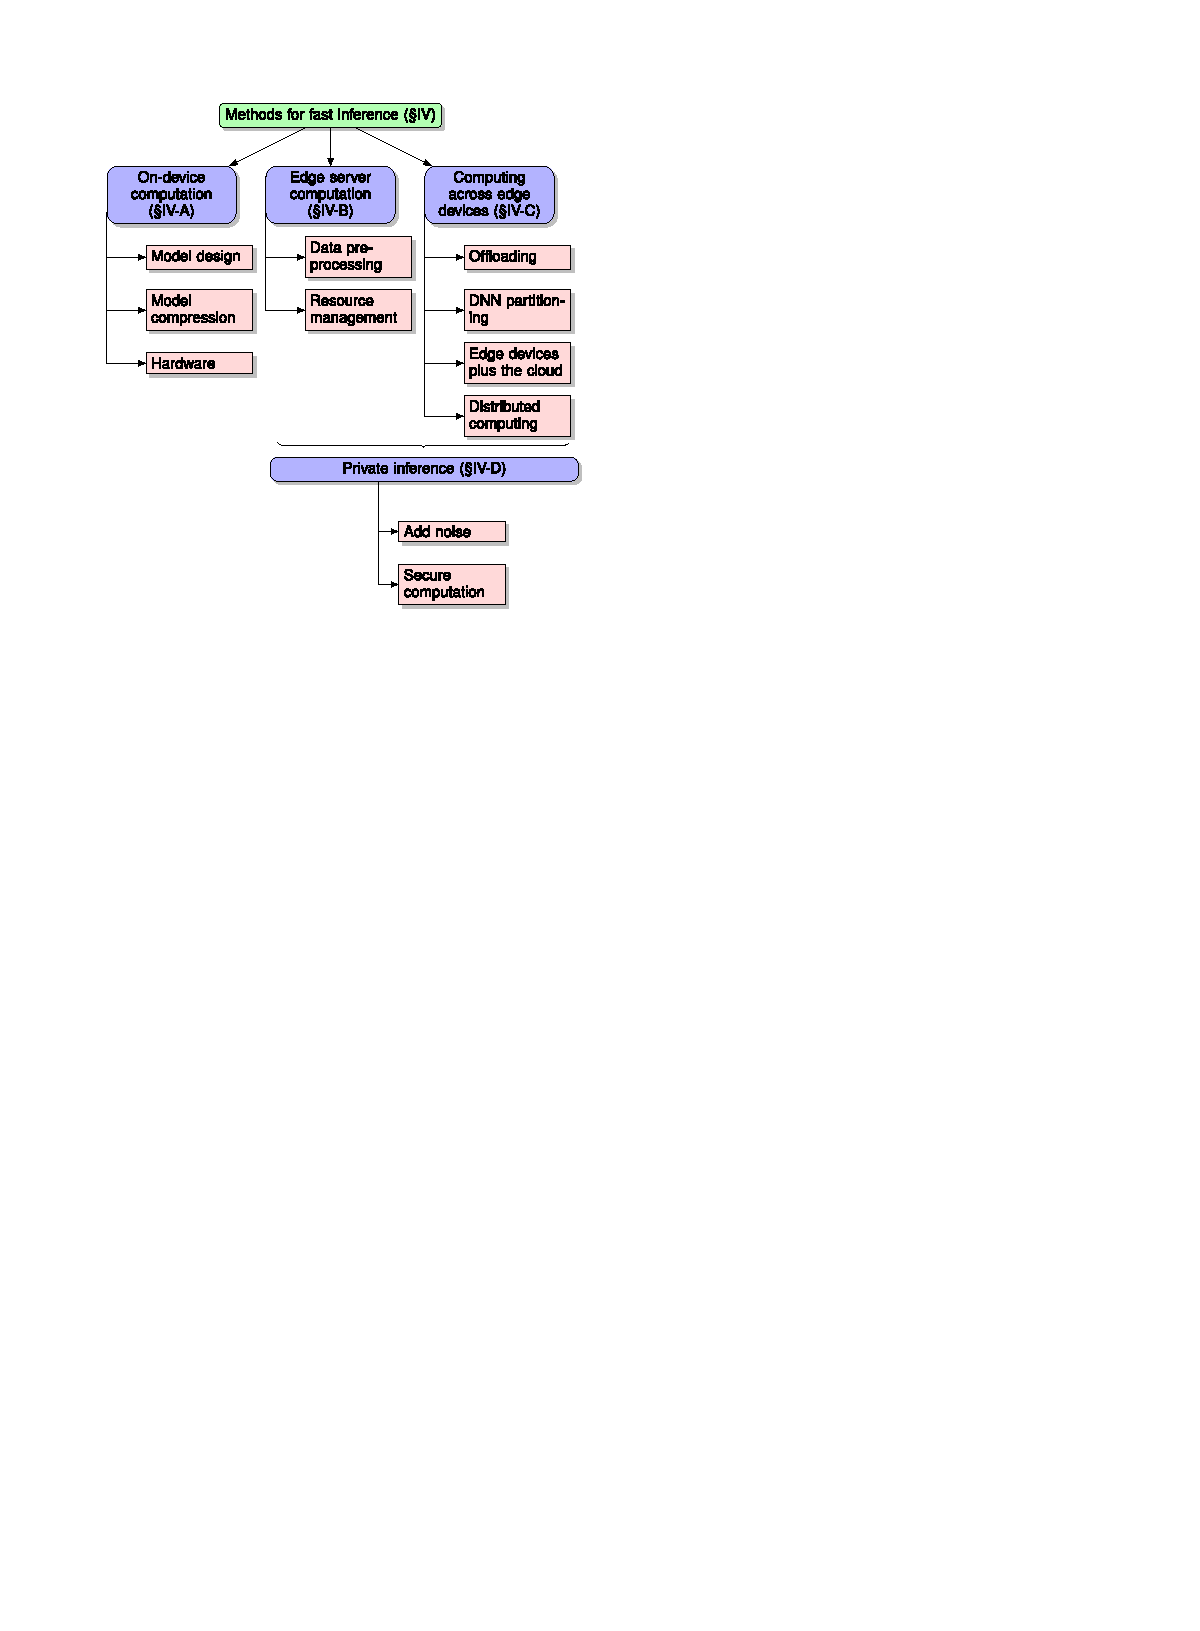
\includegraphics[scale=1]{chen2019methodsfastinference}
\caption{Methods for fast edge inference (\cite{Chen2019}).}
\end{figure}

\subsection{Deep CNN Inference on Local Devices}

In many applications, only a fixed trained model is required
to inference. The time-consuming part, training the model, can be performed offline by high-performance computing with GPU.

To achieve machine learning at the edge, two ways are identified with respect to where the computations are completed: (i) cloud-based solutions, where the data is uploaded to a the cloud and the device receives results; (ii) local computation, which contains the intelligence at the edge device. Three major weaknesses are identified for cloud-based solutions, including latency, privacy and power consumption.
Cloud-based solutions need to upload the data to the cloud, and data might be leaked during the transfer. It also depends totally on the condition of the network. If the network is not available, the application is totally non-functional. Lastly, cloud-based inference uses twice as much power compared to local processing (\cite{Lane2016}). 

\begin{table}[H]
\renewcommand{\arraystretch}{.75}
\small
\centering
\caption{Main parameters defining the architectures of the benchmarked CNN networks for 1000-category image recognition \cite{Montero2018}\cite{Hasanpour2016}}
\begin{tabular}{lcccccc}
\toprule
	&	\textbf{AlexNet}	&	\textbf{GoogLeNet}	&	\textbf{ResNet}	&	\textbf{SqueezeNet}	&	\textbf{MobileNet}	&	\textbf{SimpleNet}	\\
	& \textbf{}&\textbf{Inception-v1}	&	\textbf{50}		&	\textbf{v1.1}		&	\textbf{v1 1.0-224}	&	\textbf{v1}	\\
	\midrule
\textbf{Input}	& 224$\times$ 224 $\times$ 3 & 224$\times$ 224$\times$ 3 & 224$\times$ 224$\times$ 3 & 227$\times$ 227$\times$ 3 & 224$\times$ 224$\times$ 3 & 227$\times$ 227$\times$ 3 \\
\midrule
\textbf{CONV} \\
\# CONV layers	&		&	57	&	49	&	26	&	27	&	13	\\
\midrule
\textbf{FC} \\
\# FC Layers	&		&	1	&	1	&	0	&	1	&	1	\\
\midrule

\textbf{\# MACs}	&	724M	&	1.43G	&	3.9G \\
\textbf{Weights}	&	61M	&	$\sim$7M	&	$\sim$25.6M	&	$\sim$1.3M	&	$\sim$4.2M	&	$\sim$6.4M \\
\bottomrule
\end{tabular}
\end{table}


\begin{table}
\renewcommand{\arraystretch}{.75}
\small
\centering
\caption{Main parameters defining the architectures of the benchmarked CNN networks for 1000-category image recognition \cite{Montero2018}\cite{Hasanpour2016}}
\begin{tabular}{lccccccccc}
\toprule
\textbf{Model}	&	\textbf{MAC}	&	\textbf{CMP}	&	\textbf{ADD}	&	\textbf{DIV}	&	\textbf{ACT}	&	\textbf{Weights}	&	\textbf{Input}	&	\textbf{\# CONV}	&	\textbf{\# FC}	\\
\midrule
SimpleNet	&	1.9G	&	1.82M	&	1.5M	&	1.5M	&	6.38M	&	6.4M	&		&	13	&	1 \\
SqueezeNet	&861.34M	&	9.67M	&	226K	&	1.51M	&	12.58M	&	1.25M	&	224$\times$224$\times$3 &	26	&	0	\\
MobileNet	&			&			&			&			&			&			&	224$\times$224$\times$3	&	27	&	1	\\
ResNet-50	&	3.87G	&	10.89M	&	16.21M	&	10.59M	&	46.72M	&	25.56&	\\
AlexNet		&	7.27G	&	17.67M	&	4.78M	&	9.55M	&	20.81M	&	60.97M	&	224$\times$224$
times$3 \\
\bottomrule
\end{tabular}
\end{table}



\begin{table}
\renewcommand{\arraystretch}{.75}
\centering
\caption{ Summary of weight and MAC number of popular CNNs (\cite{Sze2017}).}
\begin{tabular}{lrrrrr}
\toprule
\textbf{Model} & \textbf{LeNet-5} &  \textbf{AlexNet} & \textbf{VGG-16} & \textbf{GoogLeNet v1} & \textbf{ResNet-50} \\
\midrule
Weights	&	60 K	&	61 M	&	138 M	&	7 M	&	25.5 M \\
MACs	&	341 K	&	724 M	&	15.5 G	&	1.43 G	&	3.9 G \\
\bottomrule
\end{tabular}
\end{table}





\begin{table}
\renewcommand{\arraystretch}{.75}
\centering
\caption{NN for edge.}
\begin{tabular}{lcl}
\toprule
\textbf{Model} & \textbf{Paper} &  \textbf{Contribution} \\
\midrule
MobileNet & \cite{Howard2017} & depthwise separable convolutions \\
ShuffleNet & \cite{Zhang2018}   & depthwise separable convolutions \\
SqueezeNet & \cite{Iandola2017} & Parameter efficiency \\
\bottomrule
\end{tabular}
\end{table}



DNN for embedded is very interesting (\cite{Iandola2017}, \cite{Zhang2017}, \cite{Lin2018}, \cite{Warden2018}, \cite{Price2018}).

MobileNet (\cite{Howard2017}) uses depthwise separable convolutions to reduce computations.

ShuffleNet (\cite{Zhang2018}) utilizes two new operations, pointwise group convolution and channel shuffle. On an ARM-based mobile device, ShuffleNet achieves 13× actual speedup over AlexNet while maintaining comparable accuracy.

\FloatBarrier

\section{IoT for Bird Detection}

\begin{table}
\renewcommand{\arraystretch}{.75}
\small
\centering
\caption{Currently available autonomous sound recorders (\cite{Darras2019}, \cite{Merchant2015}, \cite{Beason2019}). Prices shown include the additional cost of a microphone where one is not provided with the basic unit.}
\label{rpi}
\begin{tabular}{llp{2.5cm}clllllp{2cm}}
\toprule
				&				&						&	&	\multicolumn{2}{c}{\textbf{Power (mW)}}\\
\cline{5-6}
\textbf{Device} & \textbf{Cost} & \textbf{Manufacturer} & \textbf{Storage} & \textbf{Active} & \textbf{Sleep} &  \textbf{Reference} \\
\midrule
SM4BATFS	& \$1099 & Wildlife Acoustics & 512 & 155-270 & 1.8 \\
SM4			& \$1048 & Wildlife Acoustics & 512 & 135-185 & 1.8 \\
Anabat Express & \textsterling 834 & Titley Scientific & 32 & 69-113 & 3.1 \\
RPA2 		& \textsterling 210 & Peersonic & 32 & 405-605 & 30 \\
Solo 		& \textsterling 63 & $\dagger$ & 256 & 315-450 & -- &  \cite{Whytock2017} \\
Audiomoth 	& \textsterling 36 & Open Acoustic Devices & 32 & 17-70 & 0.08 & \cite{Hill2018} \\
Bat Pi 2 & -- & Fledermausschutz & 64 & -- & -- & \cite{Fledermausschutz2015} \\
Swift && Cornell & \\
-- & &Imperial College &&&& \cite{Sethi2018} \\
\bottomrule
\end{tabular}
\newline
$\dagger$ Open source
\end{table}

In automatic bioacoustic monitoring it is important to do continuous observations to capture rare events, but storage and communication overheads typically prevent continuous real- time monitoring. To overcome this limitation, this paper presents a low complexity local processing method for acoustic signals targeting resource constrained nodes and preprocessing and seg- mentation techniques in line with the proposed local processing technique for effective and continuous identification of bird calls. This paper also focuses on designing of overall automatic bioacoustic monitoring system including feature extraction and classification.
(\cite{Weerasena2019})

FPGA-based feature extraction implementation allows the system to process data from 30 acoustic sensors in real time with.
In terms of the implementation of the birdsong recognition system, the Mel scale filter bank entails the highest execution cost. Since the series implementation still shows acceptable results in terms of time consumption %\cite{Hervas2017}

Automated Remote Biodiversity Monitoring Network (ARBIMON), a novel combination of hardware and software for automating data acquisition, data management, and species identification based on audio recordings. The major components of the cyberinfrastructure include: a solar powered remote monitoring station that sends 1-min recordings every 10 min to a base station, which relays the recordings in real-time to the project server, where the recordings are processed and uploaded to the project website (arbimon.net). (\cite{Aide2013})

Others
\cite{Stowell2019}
\cite{Ovaskainen2018}


\begin{table}
\small
\centering
\caption{Bioacoustic detection algorithms.}
\label{biodetect}
\begin{tabular}{lll}
\toprule
Algorithm & Platform & Ref \\
\midrule
Goetzel filter & Audiomoth & \cite{Prince2019} \\
Bat detective & i9 & \cite{MacAodha2018} \\
\bottomrule
\end{tabular}
\end{table}

\section{Conclusion}

Outline the context of the research topic. Reflect on the research objective in light of the context, and devise an appropriate strategy.

Due to low resources, investigate methods to perform segmentation in spectrogram ROI. Then predict the class using template matching. 


\begin{table}
\renewcommand{\arraystretch}{1}
\small
\centering
\caption{ImageNet-Class CNN for bird recognition.}
\begin{tabular}{lcccccc}
\toprule
\textbf{Reference} & \textbf{Model} & \textbf{Input} & \textbf{Species Count} & \textbf{Best Accuracy} \\
\midrule
\cite{Xie2017} & VGG16 & $224\times 224$& 18 & 92.8\% \\
\bottomrule
\end{tabular}
\end{table}




\begin{table}[H]
\renewcommand{\arraystretch}{1}
\small
\centering
\caption{Custom CNN for sound recognition.}
\begin{tabular}{lcccccc}
\toprule
\textbf{Reference} & \textbf{Layers} & \textbf{Input} & \textbf{Target} & \textbf{Best Accuracy} \\
\midrule
\cite{Takahashi2016} & 9 & & Birds & 92.8\% \\
\cite{Grill2017} & && Birds & \\
\cite{Meyer2017} & 8 & & 86.0\% \\
\cite{MacAodha2018} & 4 (3 CNN, 1 FC) & $130\times 20\times 1$  & Bats & Precision 89.5\% \\
\cite{Ozer2018} & 7 (5 CNN, 2 FC) & $513\times 93\times 3$ & Sound event & 97.4\% \\
\cite{Ruff2019} & 6 (4 CNN, 2 FC) & $500\times 129\times 1$ & 7 owl species & 92.5\% \\
\bottomrule
\end{tabular}
\end{table}
